\documentclass[10pt,a4paper]{article}
\usepackage[utf8]{inputenc}
\usepackage{kotex}
\usepackage{amsmath,amssymb}
\usepackage{booktabs}
\usepackage{graphicx}
\usepackage{url}
\usepackage{caption}
\usepackage{titlesec}
\usepackage{fancyhdr}
\usepackage{geometry}
\usepackage{multicol}
\usepackage{etoolbox}

% ── KIPS 양식에 맞춘 페이지 설정 ──────────────────────────────
\geometry{
  top=2.5cm, bottom=2.5cm, left=1.5cm, right=1.5cm,
  headheight=14pt
}

% 페이지 번호 하단 중앙
\pagestyle{fancy}
\fancyhf{}
\fancyfoot[C]{\thepage}
\renewcommand{\headrulewidth}{0pt}

% 섹션 스타일: "1. 서론" 형태, 볼드, 11pt
\titleformat{\section}{\normalsize\bfseries}{\thesection.}{0.5em}{}
\titleformat{\subsection}{\normalsize\bfseries}{\thesubsection}{0.5em}{}
\titlespacing{\section}{0pt}{8pt}{4pt}
\titlespacing{\subsection}{0pt}{6pt}{3pt}

% 표/그림 캡션 작게
\captionsetup{font=small, labelfont=bf, skip=4pt}

% 단 간격
\setlength{\columnsep}{0.7cm}

% paragraph 간격
\setlength{\parindent}{1em}
\setlength{\parskip}{0pt}

\begin{document}
\thispagestyle{fancy}

% ══════════════════════════════════════════════════════════════
% 헤더 (단일 컬럼)
% ══════════════════════════════════════════════════════════════

\begin{center}
\vspace*{-0.5cm}

% 한글 제목
{\fontsize{16}{19}\selectfont\bfseries
Paraphrase Expansion Ratio 기반 텍스트 밀도 측정 및\par
트랜스포머 패러다임별 내부 처리 차이 분석\par}

\vspace{10pt}

% 저자
{\normalsize 강병수\par}
{\small 명지대학교 컴퓨터공학과 학부생\par}
\vspace{2pt}
{\small\texttt{jasonkbs@mju.ac.kr}\par}

\vspace{12pt}

% 영문 제목
{\fontsize{12}{15}\selectfont\bfseries\itshape
Text Density Measurement via Paraphrase Expansion Ratio and\par
Cross-Paradigm Analysis of Transformer Internal Processing\par}

\vspace{8pt}

% 영문 저자
{\small Byung-Soo Kang\par}
{\small Dept.\ of Computer Engineering, Myong-Ji University\par}

\vspace{14pt}

% 요약 헤더
{\normalsize\bfseries 요\qquad 약\par}
\vspace{4pt}
\end{center}

% 요약 본문 (들여쓰기 블록)
\noindent\hspace{1em}{\small%
텍스트 밀도(Text Density)는 동일한 토큰 수에 담긴 명제적 정보량의 차이를 의미하지만, 이를 정량화하는 표준적 방법은 아직 없다. 본 연구는 LLM 기반의 새로운 밀도 측정 지표인 PER(Paraphrase Expansion Ratio)을 제안하고, 6개 LLM을 통해 교차 검증한다. 또한 Encoder, Decoder, Diffusion 세 가지 트랜스포머 패러다임에서 밀도에 따른 내부 처리 차이를 분석한다. 파일럿 실험(20문장)의 결과를 확대 코퍼스(100문장)와 의미 통제된 minimal pair(100쌍)로 검증한 결과, Encoder에서는 고밀도 문장의 Layer Delta가 유의미하게 높고($p{=}0.003$), Decoder에서는 surprisal 변동계수가 유의미하게 낮으며($p{<}0.0001$), Diffusion에서는 영어 convergence area가 유의미하게 높았다($p{<}0.0001$). 이는 동일한 밀도 속성이 패러다임에 따라 서로 다른 내부 신호로 발현됨을 보여준다.\par}

\vspace{10pt}
\noindent\rule{\textwidth}{0.4pt}
\vspace{6pt}

% ══════════════════════════════════════════════════════════════
% 본문 시작 (2단)
% ══════════════════════════════════════════════════════════════
\begin{multicols}{2}

\section{서론}

자연어 텍스트에는 밀도(density)라는 속성이 존재한다. ``혁명이 숙적을 주인으로 만들지 않는다면 그것만으로도 행운이다''(부르크하르트)와 ``오늘 아침에 일찍 일어나서 따뜻한 물로 세수를 하고 밥을 먹었다''는 비슷한 토큰 수를 가지지만, 전자를 풀어쓰면 7배 이상 길어진다. 이 차이는 단순한 어휘 난이도가 아닌 명제적 압축도(propositional compression)에 기인한다.

기존의 텍스트 복잡도 측정법은 이 차이를 포착하지 못한다. Perplexity는 예측 난이도를 측정하지만 ``어려운 단어''와 ``압축된 의미''를 구분하지 못하며, 명제 밀도(propositional density)\cite{kemper1990}는 동사$\cdot$형용사 수를 세는 구조적 접근으로 암묵적 명제를 놓친다.

본 연구는 다음 세 가지 연구 질문을 다룬다. \textbf{RQ1}: PER은 서로 다른 LLM 간에도 상대적 순위를 안정적으로 보존하는가? \textbf{RQ2}: 텍스트 밀도는 패러다임별 내부 신호에 일관된 차이를 남기는가? \textbf{RQ3}: 이러한 경향은 한국어와 영어에서 어떻게 다르게 나타나는가?

\section{PER: Paraphrase Expansion Ratio}

\subsection{정의}

문장 $s$의 PER은 LLM이 생성한 풀어쓴 버전과 원문의 토큰 수 비율로 정의된다.
\begin{equation}
\mathrm{PER}(s) = \frac{|\mathrm{tokens}(\mathrm{paraphrase}(s))|}{|\mathrm{tokens}(s)|}
\end{equation}
프롬프트는 ``모든 암묵적 전제와 함축을 명시적으로 풀어 초등학생이 이해할 수 있게 재작성하라''로 통일하였다.

\subsection{교차 검증}

6개 LLM(Claude Opus/Sonnet 4.6, GPT-5.4-pro/thinking, Gemini Flash/3.1 Pro)에 대해 한국어 10문장, 영어 10문장의 PER을 산출하고 Spearman 순위 상관을 계산하였다.

GPT$\cdot$Claude 4개 모델 간 상관은 $\rho{=}0.74{\sim}0.88$\,($p{<}0.001$)로 높은 합의를 보인 반면, Gemini 계열과의 상관은 $\rho{=}{-}0.14{\sim}0.19$\,(n.s.)로 유의미하지 않았다. 이에 따라 최종 PER은 GPT$\cdot$Claude 합의 집합의 median-rank ensemble로 산출하였다.

또한 PER과 Decoder의 surprisal 변동계수 사이에 강한 음의 상관이 관찰되어(한국어 $\rho{=}{-}0.952$, $p{<}0.0001$), PER이 트랜스포머 내부의 정보 분포 균일성과 일관된 지표임을 확인하였다(RQ1).

\section{트랜스포머 내부 신호 분석}

\subsection{실험 설계}

4개 모델을 언어별로 매칭하여 사용하였다(표~\ref{tab:models}).

\vspace{4pt}
\begin{center}
\captionof{table}{실험에 사용한 모델 구성}\label{tab:models}
\footnotesize
\begin{tabular}{@{}llll@{}}
\toprule
모델 & 유형 & 언어 & 파라미터 \\
\midrule
klue/bert-base    & Enc. & KO    & 110M \\
bert-base-uncased & Enc. & EN    & 110M \\
gpt2              & Dec. & EN    & 124M \\
Qwen3-0.6B       & Dec. & KO/EN & 600M \\
\bottomrule
\end{tabular}
\end{center}
\vspace{4pt}

주요 측정 신호는 다음과 같다.

\paragraph{Layer Delta.}
연속된 레이어 간 표현 변화량이다.
\begin{equation}
\delta_l = 1 - \cos(\bar{\mathbf{h}}_l,\;\bar{\mathbf{h}}_{l-1})
\end{equation}

\paragraph{Surprisal.}
Causal LM에서 토큰 $t_i$의 정보량이다.
\begin{equation}
s(t_i) = -\log_2 P(t_i \mid t_{<i})
\end{equation}
변동계수 $\mathrm{CV}(s) = \sigma(s)/\bar{s}$는 UID 가설\cite{levy2007}의 검증 지표이다.

\paragraph{Convergence Area.}
D3PM\cite{austin2021} absorbing-state diffusion을 BERT로 근사하여, 평균 entropy 곡선의 적분값 $A = \int_0^1 \bar{H}(t)\,dt$를 측정한다.

\subsection{파일럿 실험 (20문장)}

고밀도$\cdot$저밀도 각 5문장씩으로 예비 실험을 수행하였다. klue/bert-base에서 한국어 Layer Delta가 유의미($p{=}0.032$)하였으나 영어는 n.s.였다. Surprisal CV는 한국어에서 유의미($p{=}0.008$)하였다. 이 결과를 바탕으로 검증 실험을 설계하였다.

\subsection{검증 실험 1: 확대 코퍼스}

한국어$\cdot$영어 각 50문장(고밀도 25, 저밀도 25)에서 동일 분석을 반복하였다(표~\ref{tab:general}).

\vspace{4pt}
\begin{center}
\captionof{table}{확대 코퍼스 결과 (Mann-Whitney $U$, $n$=25)}\label{tab:general}
\footnotesize
\begin{tabular}{@{}llll@{}}
\toprule
신호 & 언어 & 방향 & $p$값 \\
\midrule
Layer Delta    & KO & H${>}$L & .003** \\
Layer Delta    & EN & H${>}$L & .0001*** \\
Surp.\ Mean   & KO & H${>}$L & ${<}$.0001*** \\
Surp.\ Mean   & EN & H${>}$L & ${<}$.0001*** \\
Surp.\ CV     & KO & H${<}$L & ${<}$.0001*** \\
Surp.\ CV     & EN & H${<}$L & .003** \\
Conv.\ Area   & KO & ---     & .94\,ns \\
Conv.\ Area   & EN & H${<}$L & ${<}$.0001*** \\
\bottomrule
\end{tabular}
\end{center}
\vspace{4pt}

파일럿에서 n.s.였던 영어 Layer Delta($p{=}.0001$)와 Surprisal CV($p{=}.003$)가 표본 확대 후 유의미해졌다. 또한 한국어에서 Layer Delta와 surprisal mean 사이에 유의미한 양의 상관($\rho{=}0.378$, $p{=}.007$)이, 영어에서 surprisal mean과 convergence area 사이에 강한 음의 상관($\rho{=}{-}0.624$, $p{<}.0001$)이 관찰되어, 세 패러다임의 신호가 서로 독립이 아닌 일관된 밀도 반응 체계를 구성함을 확인하였다.

\subsection{검증 실험 2: Minimal Pairs}

교락 변수 통제를 위해 동일 의미$\cdot$다른 밀도의 minimal pair 100쌍을 구축하였다(표~\ref{tab:mp_examples}). 이는 \textbf{구문적 압축}(같은 명제의 다른 표현 길이)을 통제한다. Wilcoxon signed-rank test를 사용하였다(표~\ref{tab:minimal}).

\vspace{4pt}
\begin{center}
\captionof{table}{Minimal pair 예시 (한국어)}\label{tab:mp_examples}
\footnotesize
\begin{tabular}{@{}p{0.47\linewidth}p{0.42\linewidth}@{}}
\toprule
저밀도 (풀어쓴 표현) & 고밀도 (압축 표현) \\
\midrule
발표 전에 충분히 준비하지 않으면 질문을 받을 때 제대로 답하기 어렵다 & 준비 없는 발표는 질문 앞에서 흔들린다 \\
\addlinespace
파일을 백업하지 않은 채 시스템을 업데이트하면 중요한 문서를 잃을 수 있다 & 백업 없는 업데이트는 문서 손실을 부른다 \\
\addlinespace
창문에 생긴 작은 금을 그냥 두면 점점 커져서 결국 유리가 깨질 수 있다 & 방치한 금은 결국 유리를 깨뜨린다 \\
\bottomrule
\end{tabular}
\end{center}
\vspace{4pt}

\vspace{4pt}
\begin{center}
\captionof{table}{Minimal pair 결과 (Wilcoxon, $n$=50 pairs)}\label{tab:minimal}
\footnotesize
\begin{tabular}{@{}llll@{}}
\toprule
신호 & 언어 & 방향 & $p$값 \\
\midrule
Layer Delta    & KO & H${>}$L & .005** \\
Layer Delta    & EN & H${>}$L & ${<}$.0001*** \\
Surp.\ Mean   & KO & H${>}$L & ${<}$.0001*** \\
Surp.\ Mean   & EN & H${>}$L & ${<}$.0001*** \\
Surp.\ CV     & KO & H${<}$L & ${<}$.0001*** \\
Surp.\ CV     & EN & H${<}$L & ${<}$.0001*** \\
Conv.\ Area   & KO & ---     & .44\,ns \\
Conv.\ Area   & EN & H${<}$L & ${<}$.0001*** \\
\bottomrule
\end{tabular}
\end{center}
\vspace{4pt}

의미를 통제한 minimal pair에서도 동일 경향이 재현되었다. 이는 관찰된 차이가 어휘$\cdot$문체가 아닌 텍스트 압축 자체에 대한 모델의 반응임을 시사한다.

\subsection{표면 특성 통제}

내부 신호의 차이가 단순한 어휘$\cdot$문체 차이에 의한 것인지 확인하기 위해 probing classifier(logistic regression, LOO-CV)를 적용하였다. 모든 레이어에서 100\% 정확도를 보였으나, PCA 1개 주성분만으로도 완벽 분리가 가능하였다. 이는 고밀도(격언)와 저밀도(일상문)의 어휘 분포 차이가 크기 때문이며, Layer Delta$\cdot$Surprisal CV처럼 ``처리 방식의 차이''를 측정하는 신호와는 구별되어야 한다. 이러한 교락을 분리하기 위해 상기 minimal pair 실험을 수행하였다.

\subsection{Diffusion 결과의 언어별 비대칭}

Convergence area는 영어에서만 일관되게 유의미하였다($p{<}0.0001$). 한국어에서는 두 실험 모두 null이었으며, SOV 구조에서 iterative unmasking의 복원 순서가 밀도와 무관할 가능성이 있다.

\end{multicols}

\begin{figure}[h]
\centering
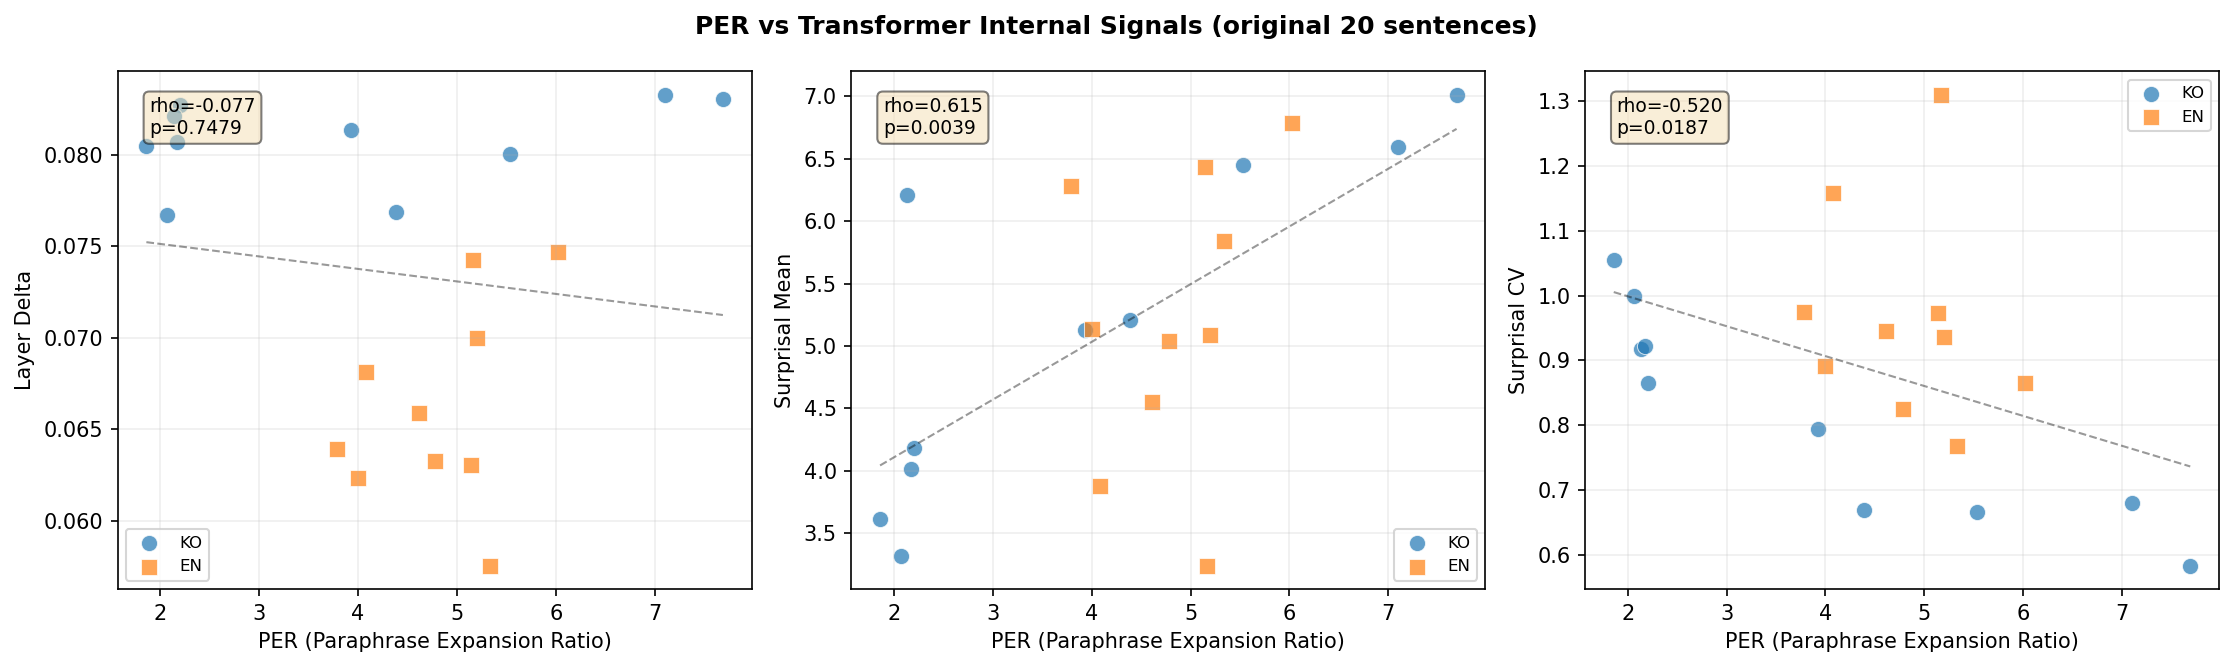
\includegraphics[width=0.95\textwidth]{fig_per_correlation.png}
\caption{PER과 트랜스포머 내부 신호 간 상관 (원본 20문장). 한국어에서 PER$\leftrightarrow$Surprisal Mean ($\rho{=}0.867$), PER$\leftrightarrow$Surprisal CV ($\rho{=}{-}0.952$)의 강한 상관이 관찰되었다.}
\label{fig:per_corr}
\end{figure}

\begin{multicols}{2}

\section{결론}

\vspace{4pt}
\begin{center}
\captionof{table}{전체 결과 요약 ($p$값, 검증 실험)}\label{tab:summary}
\footnotesize
\begin{tabular}{@{}lcccc@{}}
\toprule
 & \multicolumn{2}{c}{KO} & \multicolumn{2}{c}{EN} \\
\cmidrule(lr){2-3}\cmidrule(lr){4-5}
신호 & gen. & pair & gen. & pair \\
\midrule
Layer $\delta$  & .003** & .005** & .0001*** & ${<}$.0001*** \\
Surp.\ CV      & ${<}$.0001*** & ${<}$.0001*** & .003** & ${<}$.0001*** \\
Conv.\ $A$     & .94\,ns & .44\,ns & ${<}$.0001*** & ${<}$.0001*** \\
\bottomrule
\end{tabular}
\end{center}
\vspace{4pt}

본 연구는 텍스트 밀도가 트랜스포머 내부 처리에 패러다임별로 서로 다른 흔적을 남긴다는 것을 보였다. Encoder에서는 Layer Delta 증가로, Decoder에서는 surprisal의 균일성으로, Diffusion에서는 복원 불확실성 증가로 발현된다. 파일럿 결과는 확대 코퍼스와 minimal pair에서 재현되었다.

한계로는 minimal pair가 구문적 압축만을 통제한 점, 한국어 Diffusion 신호의 null result, BERT 기반 diffusion 근사를 사용한 점이 있다. 향후 연구에서는 (1)~명제적 밀도를 통제한 코퍼스를 추가 구축하고, (2)~PER 산출 시 프롬프트$\cdot$temperature 등 재현성 조건을 표준화하며, (3)~MDLM\cite{sahoo2024} 등 실제 diffusion language model에서 동일 분석을 반복하고, (4)~한국어 SOV 구조가 diffusion 복원 순서에 미치는 영향을 분석할 계획이다.

\begin{thebibliography}{9}
\footnotesize

\bibitem{kemper1990}
S.~Kemper \textit{et al.},
``Telling stories: The structure of adults' narratives,''
\textit{European J.\ Cognitive Psych.}, 2(3), 205--228, 1990.

\bibitem{levy2007}
R.~Levy and T.~Jaeger,
``Speakers optimize information density through syntactic reduction,''
\textit{NeurIPS}, vol.~20, 2007.

\bibitem{austin2021}
J.~Austin \textit{et al.},
``Structured denoising diffusion models in discrete state-spaces,''
\textit{NeurIPS}, vol.~34, 17981--17993, 2021.

\bibitem{sahoo2024}
S.~Sahoo \textit{et al.},
``Simple and effective masked diffusion language models,''
\textit{NeurIPS}, vol.~37, 2024.

\bibitem{kluebert}
KLUE BERT: \url{https://huggingface.co/klue/bert-base}

\bibitem{qwen2025}
Qwen Team, ``Qwen3 Technical Report,'' 2025.

\end{thebibliography}

\end{multicols}
\end{document}
